\documentclass[12pt, onepage]{article}


\usepackage[T1]{fontenc}
\usepackage{times}

\usepackage[margin=2.5cm]{geometry}
\linespread{1.5}
\usepackage{graphicx}

\usepackage[colorlinks=true,linkcolor=black,anchorcolor=black,citecolor=black,filecolor=black,menucolor=black,runcolor=black,urlcolor=black]{hyperref}
\usepackage{float}
\setlength{\parindent}{1em}
\setlength{\parskip}{1em}


%\addbibresource{bibfile.bib}
\usepackage[utf8]{inputenc}
\usepackage{amsmath}
\usepackage[export]{adjustbox}
\usepackage{wrapfig}
\usepackage{subcaption}
\usepackage{float}
\usepackage{gensymb}
\usepackage[labelfont=bf]{caption}

\numberwithin{equation}{section} %package for labelling subequations of blocks
\usepackage{listings} %package for code snippets


\pagenumbering{roman}

%tile and author
\title{How to process dual-site SETI observations with I-LOFAR and LOFAR-SE}
\date{\today}
\author{Charlie Giese}



\begin{document}
\maketitle



\linespread{1.2}

\tableofcontents
 

 
\pagenumbering{arabic}
\newpage
\linespread{1.5}

\section{Introduction}
This document is intended to instruct students in processing the data resulting from dual-site SETI observations with LOFAR-SE and I-LOFAR, as well as how the resulting data products can be compared for anti-coincidence testing. For each step of the process I will try and provide both a general explanation as well as the specific commands used. 

In order to use the data processing pipeline, you will need to modify your personal \texttt{.bashrc} file. This file is sourced by the shell upon login and essentially sets up the shell for your use. I recommend copying and pasting the last ~8 lines from \texttt{/home/charlesg/.bashrc} to your files. This will add the requisite directories to your \texttt{PATH} and other environment variables. Note, you will need to replace every instance of \texttt{\$HOME} with \texttt{/home/charlesg} in those lines. There is another useful bash script, \texttt{/usr/local/pulsar64/pulsar.bash}, which activates some of the general purpose tools installed by default on the BL machines. Note that you will need to enter \texttt{source ~/.bashrc} after doing \texttt{source /usr/local/pulsar64/pulsar.bash}. Also, activating the pulsar environment breaks something in Python, and you will need to enter \texttt{unset PYTHONPATH} to make Python work again.

In order to transfer files between the two compute nodes, I recommend using \texttt{rsync.} It has a simple syntax;\\
\noindent
\texttt{rsync [OPTIONS] user@remote1:/path/to/source \\ user@remote2:/path/to/destination}. 
This is simplest when the files you need to transfer are in the directory \texttt{/home/user} as these files can be accessed through the headnodes, \texttt{blh0}. For Onsala, you can connect to the headnode directly, but for Birr you will need to set up a multi-hop SSH connection. For details on how to do this, please see Dominic Le Duc's guide which is pinned in the interns channel on Slack.


\section{Data Processing}
\subsection{Identifying the Data}
The first processing step is to find the location of the data obtained from any one observation. Unfortunately the locations differ depending on which station you are currently using. The files we are looking for will be in Zstandard format, with a .zst file extension. These files will usually have file names like
\begin{center}
    \path{udp_SE607_16070.blc00.bl.pvt.2021-04-21T13:45:00.000.zst}
\end{center} The filename signifies the station at which it was recorded (\path{SE607} corresponds to Onsala), the date and time at which the observation began, as well as which port this file corresponds to. Our data will generally always cover 4 ports, with identifiers 0-3. As such each observation will produce 4 files named something like
\begin{center}
\path{udp_SE607_16070.blc00.bl.pvt.2021-04-21T13:45:00.000.zst}
\\
\path{udp_SE607_16071.blc00.bl.pvt.2021-04-21T13:45:00.000.zst}
\\
\path{udp_SE607_16072.blc00.bl.pvt.2021-04-21T13:45:00.000.zst}
\\
\path{udp_SE607_16073.blc00.bl.pvt.2021-04-21T13:45:00.000.zst}
\end{center}

All 4 files are required for processing to begin. At I-LOFAR, data will be found in \path{/datax2/obs/<observation_name>/udp...zst} (Note, if you're using ILISA to perform the observation the data will be located in the same directory as in the Swedish case). This data can then be accessed by logging onto blc00 and navigating to the directory in question. At the Swedish station things are a little more tricky. The file corresponding to each port is in a different directory;\\
\texttt{/datax/laneX/....} where X corresponds to the port number. On the swedish node, you can also find metadata pertaining to the observation. Metadata is found in \texttt{/datax/Projects/proj21/....} where proj21 is the project number for all SETI observations.

These .zst files are simply compressed streams of UDP packets which are produced by the station. 

\subsection{GUPPI RAW}
The ultimate goal of the processing the data is to produce two data products for every observation in the form of filterbanks. A filterbank, in this instance, a 2D stream of radio frequency channels versus time. We want to produce 2 filterbanks with varying time and frequency resolutions, one for Pulsar and FRB research, and one for SETI. A general outline of the this process can be outlined as:
\begin{itemize}
    \item Locate compressed UDP data streams
    \item Convert data in GUPPI Raw format with \path{lofar_udp_guppi_raw}
    \item Convert .raw files produced above into filterbanks using \path{rawspec}
\end{itemize}

The suite of software used in processing is all contained in a singularity image on blc00 at each station. These images are located in \path{/datax2/obs/singularity/} at both stations. 

We will first use a command-line interface (CLI) created by David McKenna called \path{lofar_udp_guppi_raw} to convert our data to GUPPI raw format. Generally this CLI can be called by simply using \texttt{lofar\_udp\_guppi\_raw -h}, to print the help options to the console for example. When using a singularity image this command becomes;\\
\texttt{singularity exec <path/to/image> lofar\_udp\_guppi\_raw -h}\\
The above command will print a help message to the console which describes the various parameters that can be passed. The images are found in \texttt{/datax2/obs/singularity} on both machines, and it's generally wise to use the most recently updated image, which at the time of writing is  \texttt{lofar-upm\_0.7.0-2021-03-25-9c91c04c3cc1.simg}. The command line arguments needed are as follows:

\begin{itemize}
    \item -i : The name of our input .zst files, with the port number replaced by \%d.
    \item -o : The output directory and name of output .raw files. General format: \texttt{<source\_name>.\%04d.raw}
    \item -m : Number of packets to process in each read request, use 4096.
    \item -e : Split the file every N iterations, use 1.
    \item -a : fakeHeader text file for observation. Based on a template you will need to provide a fakeHeader text file containing metadata to the CLI. In general, as the same frequency window will be used for each observation only the source name paramater will need to be changed. You can find a template file in /home/charlesg/B2217+47/data/ on the Swedish node.
    \item -b : Range of subbands used. 0,411 for 110-190 MHz. The exact values can be calculated based on the frequency range.
\end{itemize}
Finally, we then arrive at our completed command, except for one more modification. Currently, we need to source a bash\_profile before running the extractor, and thus our final command looks as follows. \\
\texttt{singularity exec <path/to/image>  bash -l -c \\ "source  /root/.bash\_profile;  lofar\_udp\_guppi\_raw \\ -i udp\_SE607\_1607\%d.blc00.bl.pvt.2021-04-21T13:45:00.000.zst \\
-o /output/path/B2217+47.\%04d.raw -m 4096 -e 1 \\ -a ./fakeHeader\_B2217 -b 0,411"}\\
The extractor can take some time to process our data and so it is recommend it to run it from inside a tmux virtual terminal. The process for using these is very simple. You simply enter \texttt{tmux new -s <terminal name>}, which will create a new tmux instance. You then simply execute the command in this virtual terminal. You can detach from the terminal by pressing \texttt{ctrl+B} and \texttt{D} in succesion. Re-attach to the window by entering \\ \texttt{tmux attach -t <terminal name>}. You will know that the process has exited succesfully as it will print the following message to the terminal: \\ \texttt{Data processing finished. Cleaning up file and memory objects...\\
Reader cleanup performed successfully.\\
CLI memory cleaned up successfully. Exiting.
} 


\subsection{Channelisation}
When the extractor has finished you will find many (~1-2000) .raw files in your chosen output directory. In order to form our filterbank files we use a software called \textit{rawspec}, which is a CUDA based spectroscopy package for GUPPI RAW. This process is far simpler. Navigate to your chosen output directory and enter \texttt{rawspec -f 65536,8 -t 2,16 <source\_name>} where \texttt{<source\_name>} is the same as that used above. The first argument determines the length of the FFT's (Fast Fourier Transforms). In our case, $411$ subbands become $411\times65536$ frequency channels in the case of the high frequency resolution product and $411\times8$ channels for the high time resolution production. This will produce two filterbanks (.fil extension):
\begin{itemize}
    \item \texttt{<source\_name>.rawspec.0000.fil} for the high spectral resolution product.
    \item \texttt{<source\_name>.rawspec.0001.fil} for the high time resolution product.
\end{itemize}
You can check for yourself the time and frequency resolutions of these filterbanks using Sigproc. You should be able to use Sigproc executables following the additions to your \texttt{bashrc} file earlier. 

You can use tools from Sigproc, a suite of software package used in pulsar research. It's most useful feature is the \texttt{header} command which prints the header of a specified filterbank file. It has some other tools which I recommend you check out. There also exists a Python3 wrapper for Sigproc which can be very handy, called Sigpyproc.

Once you have produced both data products at both the Irish and Swedish stations it is useful to take a brief moment to organise your directories. This is optional but I found myself often facing confusion because I hadn't named files/directories in an informative manner. Having clear and repeatable structures in your directory hierarchy will save you time in the long run.
\newpage
\section{SETI: Searching for aliens using turboSETI}
We now move onto searching our data for narrow-band signals which could be of interest to SETI researchers. To do so, we use an analysis tool called turboSETI which searches filterbank files for narrow-band signals which are drifting in frequency. turboSETI, and it's dependencies, are installed in a Python3 virtual environment, found in \texttt{/home/charlesg/seti\_py} at both stations. You can activate this environment by entering \texttt{source /home/charlesg/seti\_py/bin/activate}. Once you have activated the environment you can use turboSETI. This is quite straight-forward, simply navigate to the directory containing your high spectral resolution filterbank, and turboSETI can be called from the command line. It takes a number of arguments;
\begin{itemize}
    \item -M : Maximum drift rate for turboSETI to search to. Based on estimates by Sheikh et al. (2019) a maximum drift rate of $\pm$ 4 Hz/s is appropriate.
    \item -n : Number of coarse channels. This argument is required for turboSETI to work with our data. The number of coarse channels is simply the number of subbands before channelisation, 411 in the above example. 
    \item -s : Minimum SNR threshold. 
\end{itemize}
The final argument is then the name of the filterbank. turboSETI can also take some time to run, so using tmux is recommended. As turboSETI runs it prints the SNR and drift rate of each fit it finds to the terminal, and will print the total search time when it has finished. When turboSETI has concluded, there will be three new files in your directory. turboSETI first creates a copy of the filterbank in H5 format, with a .h5 extension, and then searches this file. It tabulates the results in a .dat file and produces a .log file which is useful for diagnostics. The .dat file is most important, it details the frequency, drift rate and SNR of each potential "hit" (narrow-band signal) turboSETI has found. It should look something like Figure \ref{fig:dat}. For each hit, you can produce a plot by calculating the central frequency of the hit and plotting a frequency window corresponding to how far the signal drifts over the length of the observation. This can be done using some of the code in my GitHub repository. Such a plot should look something like Figure \ref{fig:hit}.

\begin{figure}
    \centering
    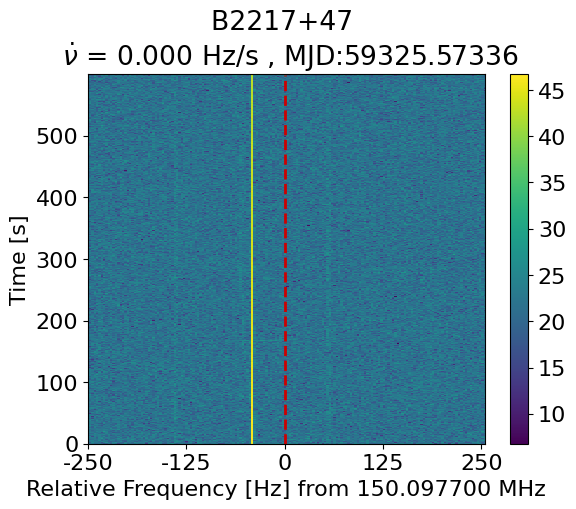
\includegraphics[width =0.6\linewidth]{94.png}
    \caption{Plot of a narrow-band hit detected by the turboSETI algorithm. For a hit which isn't drifting, a 500 Hz frequency window is standard. The dotted red line is overplotted for signals where the drift rate is difficult to see. }
    \label{fig:hit}
\end{figure}

\begin{figure}
    \centering
    \includegraphics[width = \linewidth]{Screenshot from 2021-06-13 19-37-31.png}
    \caption{Example of a .dat file output from a narrow-band search using turboSETI.}
    \label{fig:dat}
\end{figure}

Once you have done this for each station, we can begin to reject hits by comparing the results from Ireland and Sweden. For this, you will need to transfer one .dat file to another station, I recommend the Swedish station. You can do this using \texttt{rsync}. Once you have both .dat files in one directory you use a simple script to compare them. In essence, we are looking for hits which appear at the same frequency and drift rate at both stations. You can use my script \texttt{dat\_comp.py} as a basis. 

\section{SPANDAK}
For each observation a high-time resolution filterbank is also produced. These filterbanks will be searched using Heimdall, a GPU accelerated transient detection pipeline. We will also use a wrapper for Heimdall called SPANDAK which was written by Vishal Gajjar \footnote{\url{https://github.com/gajjarv/PulsarSearch}}. Using this wrapper is very straightforward, but requires some setup. Both Heimdall and SPANDAK, and their dependencies, have been installed on the compute nodes at both stations.  Every time you wish to use SPANDAK you will need to enter the following commands;
\begin{itemize}
    \item \texttt{source /usr/local/pulsar64/pulsar.bash}
    \item \texttt{source ~/.bashrc}
    \item \texttt{SPANDAK --fil file.fil --lodm 0 --hidm 10000}
\end{itemize}
(Of course you only need to enter the first two lines once, you can then run SPANDAK as many times as needed). The first command gives you access to some of the dependencies SPANDAK requires, however it overwrites some changes your \texttt{bashrc} makes and so you will need to source this again. The SPANDAK command given above will look for transients at dispersion measures from 0 to 10,000. SPANDAK will produce a .png file with some plots for each potential FRB candidate. They should look something like Figure \ref{fig:my_label} and are useful for further analysis.

\begin{figure}
    \centering
    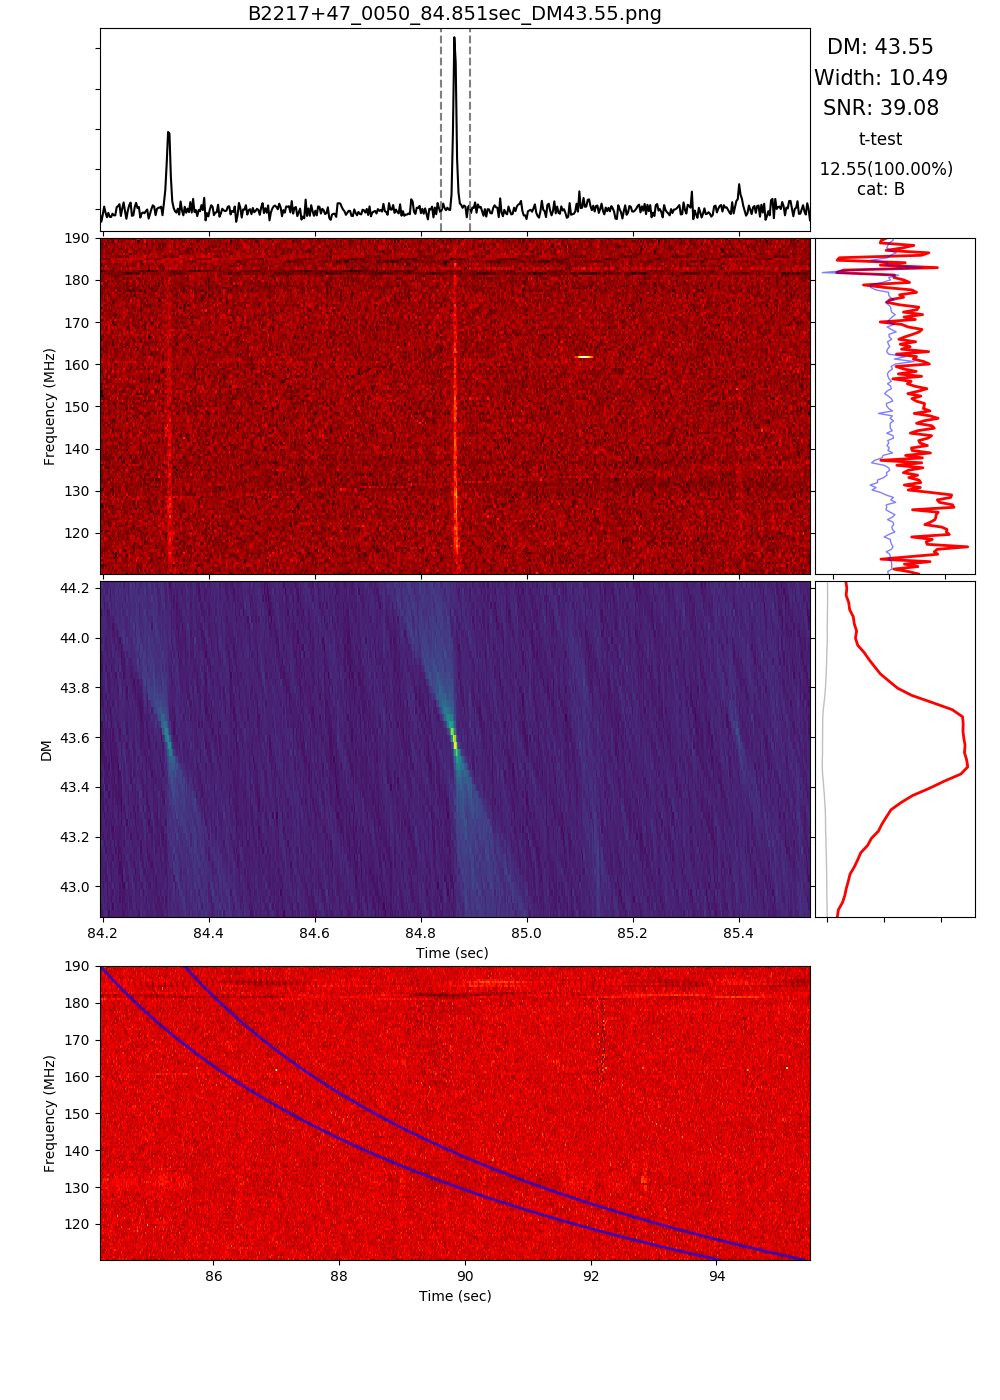
\includegraphics[width=0.8\linewidth]{B_0050_84.851sec_DM43.55.png}
    \caption{Output image of a pulse detected by the SPANDAK pipeline. Note, this image was produced using data from the pulsar B2217+47. The top panel shows a timeseries and gives some basic info about the nature of the pulse. The second panel shows a dynamic spectrum which has been dedispersed, and the panel below this shows a dispersion measure vs time spectrum. This plot shows the SNR of the pulse when dedispersed at different dispersion measures. The final panel displays a dynamic spectrum, note the quadratic shape of the pulse.}
    \label{fig:my_label}
\end{figure}


\end{document}